\documentclass[14pt,fleqn]{extarticle}
\usepackage[T2A,T1]{fontenc}
\usepackage[utf8]{inputenc}
\usepackage[russian]{babel}
\usepackage{amsmath}
\usepackage{graphicx}
\usepackage{tabularx}
\usepackage{boldline}
\usepackage{makecell}
\usepackage{arydshln}
\usepackage{mathtools}
\usepackage[a4paper, total={6.5in, 9.5in}]{geometry}

\graphicspath{ {../assets/} }
\setlength{\mathindent}{0pt}
\setlength\parindent{0pt}


\begin{document}
	\begin{titlepage}
		
\includegraphics[scale=0.12]{logo}
		\begin{center}
			\textbf{МИНОБРНАУКИ РОССИИ}\\
			\vspace{0.2cm}
			\textbf{Федеральное государственное бюджетное образовательное учреждение высшего образования}\\
			\textbf{«САНКТ-ПЕТЕРБУРГСКИЙ ГОСУДАРСТВЕННЫЙ ЭКОНОМИЧЕСКИЙ УНИВЕРСИТЕТ»}\\
			\vspace{0.6cm}
			Факультет информатики и прикладной математики\\
			Кафедра прикладной математики и экономико-математических методов\\
			\vspace{1cm}
			\textbf{ОТЧЁТ}\\
			по дисциплине:\\
			\textbf{«Теория и системы поддержки принятия решений»}\\
			на тему:\\
			\textbf{«Многокритериальная линейная оптимизация. Задание 1»}\\
		\end{center}
		\vspace{1cm}
		Направление: 01.03.02\\
		Обучающийся: Бронников Егор Игоревич\\
		Группа: ПМ-1901\\
		\vfill
		\begin{center}
			Санкт-Петербург\\
			2022\\
		\end{center}
	\end{titlepage}
	\section*{Задача 1}
	\textit{Критерии:}\\
	$f_1 = x_1 + x_2 + 2 \longrightarrow max$\\
	$f_2 = x_1 - x_2 + 6 \longrightarrow max$\\
	
	\textit{Ограничения:}
	\begin{align*}
		\begin{cases}
			x_1 + 2x_2 \leq 6\\
			0 \leq x_1 \leq 4\\
			0 \leq x_2 \leq 2\\
		\end{cases}
	\end{align*}
	
	\textit{Найти \underline{компромиссное решение}}\\
	
	1) Находим индивидуальные экстремальные значения рассматриваемых критериев:
	\begin{center}
		$max f_1 = 7, \hspace{0.45cm} x_1 = 4, \hspace{0.2cm} x_2 = 1: \hspace{0.2cm} f_2 = 9$\\
		$max f_2 = 10, \hspace{0.2cm} x_1 = 4, \hspace{0.2cm} x_2 = 0: \hspace{0.2cm} f_1 = 6$
	\end{center}

	2) Введём компромиссную переменную $z$ и сформулируем неравенства для относительных отклонений:
	\begin{center}
		$f_1: \hspace{0.2cm} x_1 + x_2 + 2 + 7z \geq 7$\\
		$\hspace{0.52cm} f_2: \hspace{0.2cm} x_1 - x_2 + 6 + 10z \geq 10$\\
		$z \geq 0$
	\end{center}
	3) Формулируем вспомогательную целевую функцию:
	\begin{center}
		$F = z \longrightarrow min$
	\end{center}
	4) Решаем задачу оптимизации:\\
	
	Целевая функция:\\
	$F = z \longrightarrow min$\\
	
	Ограничения:
	\begin{align*}
		\begin{cases}
			x_1 + 2x_2 \leq 6\\
			0 \leq x_1 \leq 4\\
			0 \leq x_2 \leq 2\\
			x_1 + x_2 + 2 + 7z \geq 7\\
			x_1 - x_2 + 6 + 10z \geq 10\\
			z \geq 0\\
		\end{cases}
	\end{align*}
	\newpage
	Её решение имеет вид:
	\begin{center}
		$z^* = 0.0588235, \hspace{0.2cm} x_1^* = 4, \hspace{0.2cm} x_2^* = 0.0588235: \hspace{0.2cm} f_1^* = 6.58824 \hspace{0.2cm} f_2^* = 9.41177$
	\end{center}
	Таким образом, мы получили эффективное решение. Значение $z^*$ показывает, что относительные отклонения компромиссных значений критериев $f_1$ и $f_2$ от их оптимальных величин $f_{1, max}$ и $f_{2, max}$ не превышает 6\%, что хорошо:
	\begin{center}
		$f_{1, max} = 7, \hspace{0.2cm} f_{2, max} = 10$
	\end{center}
	\textbf{Ответ:} $x_1^* = 4, \hspace{0.2cm} x_2^* = 0.0588235: \hspace{0.2cm} f_1^* = 6.58824, \hspace{0.2cm} f_2^* = 9.41177$
	
	\section*{Задача 2}
	\textit{Критерии:}\\
	$f_1 = x_1 + x_2 + 2 \longrightarrow max$\\
	$f_2 = x_1 - x_2 + 6 \longrightarrow max$\\
	
	\textit{Ограничения:}
	\begin{align*}
		\begin{cases}
			x_1 + 2x_2 \leq 6\\
			0 \leq x_1 \leq 4\\
			0 \leq x_2 \leq 2\\
		\end{cases}
	\end{align*}
	
	Критерий $f_1 -$ главный и уступка $p_1 = 10\%$\\
	
	\textit{Найти решение \underline{методом последовательных уступок (методом главного}\\
	\underline{критерия)}}\\
	
	1) Находим индивидуальные экстремальные значения рассматриваемых критериев:
	\begin{center}
		$max f_1 = 7, \hspace{0.45cm} x_1 = 4, \hspace{0.2cm} x_2 = 1: \hspace{0.2cm} f_2 = 9$\\
		$max f_2 = 10, \hspace{0.2cm} x_1 = 4, \hspace{0.2cm} x_2 = 0: \hspace{0.2cm} f_1 = 6$
	\end{center}
	2) Получаем дополнительное ограничение для $f_1$:
	\begin{center}
		$f_1: \hspace{0.2cm} x_1 + x_2 + 2 \geq 7 \times (1-0.1) = 6.3$
	\end{center}
	\newpage
	3) Решаем задачу максимизации для $f_2$ с исходными ограничениями и с дополнительным ограничением:\\
	
	Целевая функция:\\
	$f_2 = x_1 - x_2 + 6 \longrightarrow max$\\
	
	Ограничения:
	\begin{align*}
		\begin{cases}
			x_1 + 2x_2 \leq 6\\
			0 \leq x_1 \leq 4\\
			0 \leq x_2 \leq 2\\
			x_1 + x_2 + 2 \geq 6.3\\
		\end{cases}
	\end{align*}

	\textbf{Ответ:} $x_1^* = 4, \hspace{0.2cm} x_2^* = 0.3: \hspace{0.2cm} f_1^* = 6.3, \hspace{0.2cm} f_2^* = 9.7$
	
	\section*{Задача 3}
	\textit{Критерии:}\\
	$f_1 = x_1 + x_2 + 2 \longrightarrow max$\\
	$f_2 = x_1 - x_2 + 6 \longrightarrow max$\\
	
	\textit{Ограничения:}
	\begin{align*}
		\begin{cases}
			x_1 + 2x_2 \leq 6\\
			0 \leq x_1 \leq 4\\
			0 \leq x_2 \leq 2\\
		\end{cases}
	\end{align*}
	
	Уступка $p_1$ для первого критерия $f_1$ составляет 5, 10 и 15\%\\
	Уступка $p_2$ для второго критерия $f_2$ равна 10, 15 и 20\%\\
	
	\textit{Найти решение \underline{методом последовательных уступок (случай двух критериев)}}\\
	
	1) Находим индивидуальные экстремальные значения рассматриваемых критериев:
	\begin{center}
		$max f_1 = 7, \hspace{0.45cm} x_1 = 4, \hspace{0.2cm} x_2 = 1: \hspace{0.2cm} f_2 = 9$\\
		$max f_2 = 10, \hspace{0.2cm} x_1 = 4, \hspace{0.2cm} x_2 = 0: \hspace{0.2cm} f_1 = 6$
	\end{center}
	\newpage
	2) При максимизации $f_1$ уступка по $f_2$ приводит к следующему ограничению:
	\begin{center}
		$f_2: \hspace{0.2cm} x_1 - x_2 + 6 \geq 10 \times (1 - p_2)$
	\end{center}
	При максимизации $f_2$ уступка по $f_1$ приводит к следующему ограничению:
	\begin{center}
		$f_1: \hspace{0.2cm} x_1 + x_2 + 2 \geq 7 \times (1 - p_1)$
	\end{center}
	
	\begin{center}
		\begin{tabular}{p{6cm} p{3cm}}
			$f_1 \longrightarrow max$: & $f_2 \longrightarrow max$:\\
			\begin{tabular}{ |c|c|c| }
				\hline
				$p_2$ для $f_2$ & $f_1$ & $f_2$\\
				\hline
				0 & 6 & 10\\
				\hline
				0.03 & 6.3 & 9.7\\
				\hline
				0.05 & 6.5 & 9.5\\
				\hline
				0.08 & 7 & 9\\
				\hline
				0.1 & 7 & 9\\
				\hline
				0.15 & 7 & 9 \\
				\hline
				0.2 & 7 & 9\\
				\hline
			\end{tabular} &
			\begin{tabular}{ |c|c|c| }
				\hline
				$p_1$ для $f_1$ & $f_1$ & $f_2$\\
				\hline
				0 & 7 & 9\\
				\hline
				0.05 & 6.65 & 9.35 \\
				\hline
				0.1 & 6.3 & 9.7 \\
				\hline
				0.15 & 6 & 10 \\
				\hline
			\end{tabular} \\
		\end{tabular}
	\end{center}
	\begin{center}
		\textit{Таблица 1}. Метод последовательных уступок II
	\end{center}
	\begin{center}
		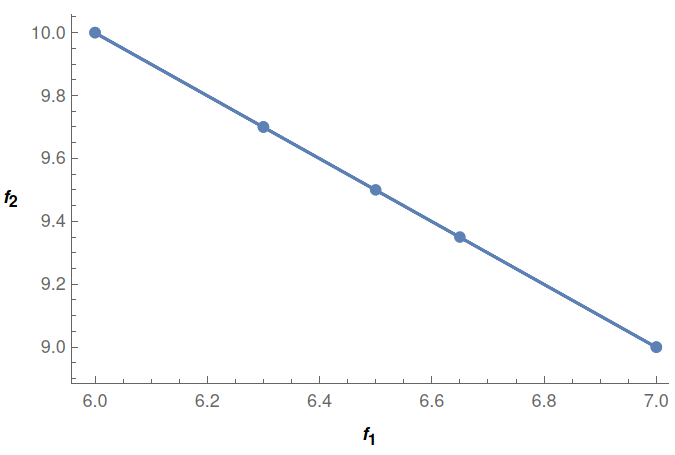
\includegraphics[scale=0.45]{plot}
	\end{center}
	\begin{center}
		\textit{Рис. 1}. График зависимости $f_2$ от $f_1$
	\end{center}
	Теперь лицо принимающее решение может выбрать любую точку на этом графике.
	\newpage
	
	\section*{Задача 4}
	\textit{Критерии:}\\
	$f_1 = x_1 + x_2 + 2 \longrightarrow max$\\
	$f_2 = x_1 - x_2 + 6 \longrightarrow max$\\
	
	\textit{Ограничения:}
	\begin{align*}
		\begin{cases}
			x_1 + 2x_2 \leq 6\\
			0 \leq x_1 \leq 4\\
			0 \leq x_2 \leq 2\\
		\end{cases}
	\end{align*}
	
	\textit{Найти решение многоритериальной задачи с двумя целевыми функциями \underline{методом равных и наименьших отклонений}}\\
	
	1) Находим индивидуальные экстремальные значения рассматриваемых критериев:
	\begin{center}
		$max f_1 = 7, \hspace{0.45cm} x_1 = 4, \hspace{0.2cm} x_2 = 1: \hspace{0.2cm} f_2 = 9$\\
		$max f_2 = 10, \hspace{0.2cm} x_1 = 4, \hspace{0.2cm} x_2 = 0: \hspace{0.2cm} f_1 = 6$
	\end{center}

	2) Переписываем два критерия:
	\begin{center}
		$x_1 + x_2 + 2 - f_1 = 0$\\
		$x_1 - x_2 + 6 - f_2 = 0$
	\end{center}
	$f_1$ и $f_2$ теперь рассматриваем как дополнительные переменные\\
	
	3) Записываем дополнительное соотношение (условие равенства отклонений):
	\begin{center}
		$\dfrac{x_1 + x_2 + 2}{7} - \dfrac{x_1 - x_2 + 6}{10} = 0$
	\end{center}

	\newpage
	
	4) Формулируем и решаем замещающую задачу ($f_1$ выбираем в качестве целевой функции):\\
	
	Целевая функция:\\
	$f_1 = x_1 + x_2 + 2 \longrightarrow max$\\
	
	Ограничения:
	\begin{align*}
		\begin{cases}
			x_1 + 2x_2 \leq 6\\
			0 \leq x_1 \leq 4\\
			0 \leq x_2 \leq 2\\
			\dfrac{x_1 + x_2 + 2}{7} - \dfrac{x_1 - x_2 + 6}{10} = 0\\
		\end{cases}
	\end{align*}
	\textbf{Ответ:} $x_1^* = 4, \hspace{0.2cm} x_2^* = 0.5882: \hspace{0.2cm} f_1^* = 6.5882, \hspace{0.2cm} f_2^* = 9.4118$
	
	\section*{Задача 5}
	\textit{Критерии:}\\
	$f_1 = x_1 + x_2 + 2 \longrightarrow max$\\
	$f_2 = x_1 - x_2 + 6 \longrightarrow max$\\
	
	\textit{Ограничения:}
	\begin{align*}
		\begin{cases}
			x_1 + 2x_2 \leq 6\\
			0 \leq x_1 \leq 4\\
			0 \leq x_2 \leq 2\\
		\end{cases}
	\end{align*}

	\textit{Найти решение многоритериальной задачи с двумя целевыми функциями \underline{методом весовых оценок критериев (метод экспертных оценок)}}\\
	
	1) Задаём значения весовых коэффициентов:
	\begin{center}
		$\alpha_1 = 0.7, \hspace{0.2cm} \alpha_2 = 0.3: \hspace{0.5cm} \alpha_1 + \alpha_2 = 1$\\
	\end{center}
	2) Формулируем обобщающую целевую функцию:
	\begin{center}
		$F = \alpha_1 f_1 + \alpha_2 f_2 = 0.7(x_1 + x_2 + 2) + 0.3(x_1 - x_2 + 6) \longrightarrow max$\\
	\end{center}
	\newpage
	3) Решаем задачу оптимизации:\\
	
	Целевая функция:\\
	$F = 0.7(x_1 + x_2 + 2) + 0.3(x_1 - x_2 + 6) \longrightarrow max$\\
	
	Ограничения:
	\begin{align*}
		\begin{cases}
			x_1 + 2x_2 \leq 6\\
			0 \leq x_1 \leq 4\\
			0 \leq x_2 \leq 2\\
		\end{cases}
	\end{align*}
	\textbf{Ответ:} $ F^* = 7.6, \hspace{0.2cm} x_1^* = 4, \hspace{0.2cm} x_2^* = 1: \hspace{0.2cm} f_1^* = 7, \hspace{0.2cm} f_2^* = 9$
	
	\section*{Сводный результат}
	\begin{center}
			\begin{tabular}{|c|c|c|c|c|}
			\hline
			& $f_1$ & $f_2$ & $x_1$ & $x_2$\\
			\hline
			$f_1 \longrightarrow max$ & 7 & 9 & 4 & 1\\
			\hline
			$f_2 \longrightarrow max$ & 10 & 6 & 4 & 0\\
			\hline
			\small Задача 1 \normalsize & 6.58824 & 9.41177 & 4 & 0.0588235\\
			\hline
			\small Задача 2 \normalsize & 6.3 & 9.7 & 4 & 0.3\\
			\hline
			\small Задача 4 \normalsize & 6.5882 & 9.4118 & 4 & 0.5882\\
			\hline
			\small Задача 5 \normalsize & 7 & 9 & 4 & 1\\
			\hline
		\end{tabular}
	\end{center}
\end{document}